\begin{table*}[!htbp]
\centering
\caption{1DSfM Notre Dame, 100-camera sub-graphs, calibration and test cameras disjoint; 5 seeds $\times$ 20 test scenes. Same conventions as \cref{tab:synth}; with 5 seeds no comparison can reach the marker threshold.}
\label{tab:real}
\setlength{\tabcolsep}{3.2pt}
\footnotesize
\begin{adjustbox}{max width=\textwidth,max totalheight=0.85\textheight}\begin{tabular}{llcccccc}
\toprule
Condition & Method & AUC@2$^\circ\uparrow$ & AUC@5$^\circ\uparrow$ & Med.\ ($^\circ$)$\downarrow$ & P95 ($^\circ$)$\downarrow$ & Reg.\ (\%)$\uparrow$ & Cat.\ (\%)$\downarrow$\\
\midrule
Clean & L1 & 0.562\,{\scriptsize[0.543,0.590]} & 0.764\,{\scriptsize[0.749,0.782]} & 0.64 & 6.1 & 100.0 & 0.4\\
 & CG & 0.559\,{\scriptsize[0.537,0.589]} & \textbf{0.768\,{\scriptsize[0.752,0.788]}} & 0.67 & 6.1 & 100.0 & 0.6\\
 & CycFilt & 0.559\,{\scriptsize[0.537,0.590]} & 0.768\,{\scriptsize[0.753,0.787]} & 0.66 & 6.1 & 99.9 & 0.7\\
 & GLOMAP-RA & 0.557\,{\scriptsize[0.534,0.588]} & 0.765\,{\scriptsize[0.749,0.785]} & 0.66 & 5.7 & 99.5 & 0.8\\
 & Shonan-H & 0.515\,{\scriptsize[0.495,0.539]} & 0.742\,{\scriptsize[0.727,0.761]} & 0.78 & 7.6 & 100.0 & 0.6\\
 & CG-$\hat\rho$ & 0.555\,{\scriptsize[0.532,0.583]} & 0.767\,{\scriptsize[0.751,0.786]} & 0.68 & 6.1 & 100.0 & 0.6\\
 & CARA-static & 0.550\,{\scriptsize[0.526,0.580]} & 0.742\,{\scriptsize[0.718,0.766]} & 0.60 & 3.9 & 92.1 & 8.1\\
 & CARA & 0.547\,{\scriptsize[0.522,0.576]} & 0.743\,{\scriptsize[0.720,0.765]} & 0.62 & 3.9 & 92.4 & 7.7\\
 & CARA-safe & 0.516\,{\scriptsize[0.493,0.544]} & 0.732\,{\scriptsize[0.710,0.753]} & 0.71 & 4.0 & 93.4 & 6.7\\
\midrule
Noise $\kappa{=}1.5$ & L1 & 0.422\,{\scriptsize[0.401,0.448]} & 0.682\,{\scriptsize[0.661,0.703]} & 1.04 & 6.9 & 100.0 & 0.3\\
 & CG & 0.439\,{\scriptsize[0.418,0.463]} & 0.693\,{\scriptsize[0.671,0.716]} & 0.98 & 7.2 & 100.0 & 0.5\\
 & CycFilt & 0.439\,{\scriptsize[0.418,0.463]} & 0.693\,{\scriptsize[0.671,0.715]} & 0.98 & 7.2 & 99.9 & 0.6\\
 & GLOMAP-RA & 0.440\,{\scriptsize[0.419,0.463]} & \textbf{0.694\,{\scriptsize[0.672,0.715]}} & 0.98 & 6.3 & 99.4 & 1.0\\
 & Shonan-H & 0.428\,{\scriptsize[0.410,0.450]} & 0.687\,{\scriptsize[0.667,0.708]} & 1.02 & 6.6 & 100.0 & 0.3\\
 & CG-$\hat\rho$ & 0.415\,{\scriptsize[0.395,0.435]} & 0.678\,{\scriptsize[0.657,0.699]} & 1.06 & 6.9 & 100.0 & 0.4\\
 & CARA-static & 0.435\,{\scriptsize[0.414,0.460]} & 0.670\,{\scriptsize[0.642,0.697]} & 0.87 & 5.1 & 89.6 & 10.7\\
 & CARA & 0.414\,{\scriptsize[0.393,0.435]} & 0.670\,{\scriptsize[0.646,0.693]} & 1.00 & 5.5 & 95.2 & 4.8\\
 & CARA-safe & 0.398\,{\scriptsize[0.378,0.420]} & 0.658\,{\scriptsize[0.634,0.682]} & 1.06 & 5.5 & 95.2 & 4.8\\
\midrule
Noise $\kappa{=}3$ & L1 & 0.297\,{\scriptsize[0.281,0.312]} & 0.590\,{\scriptsize[0.568,0.613]} & 1.50 & 8.0 & 100.0 & 0.3\\
 & CG & 0.258\,{\scriptsize[0.243,0.274]} & 0.557\,{\scriptsize[0.534,0.579]} & 1.68 & 9.0 & 100.0 & 0.3\\
 & CycFilt & 0.258\,{\scriptsize[0.243,0.274]} & 0.557\,{\scriptsize[0.535,0.581]} & 1.68 & 9.0 & 100.0 & 0.4\\
 & GLOMAP-RA & 0.261\,{\scriptsize[0.246,0.276]} & 0.561\,{\scriptsize[0.539,0.584]} & 1.66 & 8.6 & 99.6 & 0.6\\
 & Shonan-H & 0.302\,{\scriptsize[0.287,0.318]} & \textbf{0.596\,{\scriptsize[0.573,0.619]}} & 1.48 & 8.0 & 100.0 & 0.3\\
 & CG-$\hat\rho$ & 0.298\,{\scriptsize[0.282,0.314]} & 0.591\,{\scriptsize[0.566,0.615]} & 1.51 & 8.0 & 100.0 & 0.3\\
 & CARA-static & 0.152\,{\scriptsize[0.120,0.181]} & 0.318\,{\scriptsize[0.250,0.380]} & 2.24 & 4.7 & 49.0 & 51.0\\
 & CARA & 0.298\,{\scriptsize[0.282,0.314]} & 0.587\,{\scriptsize[0.562,0.613]} & 1.45 & 6.8 & 96.0 & 4.1\\
 & CARA-safe & 0.289\,{\scriptsize[0.272,0.306]} & 0.580\,{\scriptsize[0.554,0.605]} & 1.48 & 6.9 & 95.8 & 4.2\\
\midrule
+15\% outl. & L1 & 0.536\,{\scriptsize[0.515,0.560]} & 0.739\,{\scriptsize[0.721,0.757]} & 0.70 & 15.1 & 100.0 & 2.4\\
 & CG & 0.546\,{\scriptsize[0.524,0.571]} & \textbf{0.753\,{\scriptsize[0.733,0.773]}} & 0.69 & 13.8 & 100.0 & 2.3\\
 & CycFilt & 0.538\,{\scriptsize[0.516,0.564]} & 0.742\,{\scriptsize[0.721,0.762]} & 0.68 & 8.3 & 97.5 & 4.0\\
 & GLOMAP-RA & 0.544\,{\scriptsize[0.522,0.569]} & 0.750\,{\scriptsize[0.731,0.769]} & 0.68 & 12.1 & 99.0 & 3.0\\
 & Shonan-H & 0.492\,{\scriptsize[0.473,0.515]} & 0.724\,{\scriptsize[0.706,0.742]} & 0.84 & 16.3 & 100.0 & 2.3\\
 & CG-$\hat\rho$ & 0.528\,{\scriptsize[0.505,0.554]} & 0.747\,{\scriptsize[0.726,0.768]} & 0.74 & 13.4 & 100.0 & 2.3\\
 & CARA-static & 0.537\,{\scriptsize[0.514,0.562]} & 0.726\,{\scriptsize[0.702,0.750]} & 0.61 & 6.7 & 90.0 & 10.3\\
 & CARA & 0.522\,{\scriptsize[0.499,0.549]} & 0.725\,{\scriptsize[0.706,0.748]} & 0.67 & 8.5 & 91.7 & 8.8\\
 & CARA-safe & 0.474\,{\scriptsize[0.450,0.498]} & 0.700\,{\scriptsize[0.677,0.725]} & 0.81 & 7.5 & 92.8 & 7.6\\
\midrule
$\kappa{=}1.5$+15\% & L1 & 0.387\,{\scriptsize[0.363,0.410]} & 0.650\,{\scriptsize[0.626,0.673]} & 1.17 & 14.3 & 100.0 & 2.7\\
 & CG & 0.424\,{\scriptsize[0.400,0.453]} & 0.675\,{\scriptsize[0.653,0.697]} & 1.03 & 14.3 & 100.0 & 2.5\\
 & CycFilt & 0.420\,{\scriptsize[0.396,0.444]} & 0.666\,{\scriptsize[0.641,0.690]} & 1.01 & 11.0 & 97.5 & 4.3\\
 & GLOMAP-RA & 0.424\,{\scriptsize[0.400,0.450]} & \textbf{0.675\,{\scriptsize[0.652,0.698]}} & 1.02 & 17.3 & 99.4 & 3.1\\
 & Shonan-H & 0.407\,{\scriptsize[0.382,0.436]} & 0.666\,{\scriptsize[0.645,0.689]} & 1.10 & 16.6 & 100.0 & 2.3\\
 & CG-$\hat\rho$ & 0.390\,{\scriptsize[0.365,0.416]} & 0.655\,{\scriptsize[0.634,0.676]} & 1.17 & 13.1 & 100.0 & 2.3\\
 & CARA-static & 0.419\,{\scriptsize[0.394,0.447]} & 0.647\,{\scriptsize[0.618,0.676]} & 0.87 & 5.3 & 85.5 & 14.8\\
 & CARA & 0.389\,{\scriptsize[0.365,0.418]} & 0.646\,{\scriptsize[0.621,0.671]} & 1.07 & 6.6 & 93.3 & 7.0\\
 & CARA-safe & 0.368\,{\scriptsize[0.343,0.396]} & 0.629\,{\scriptsize[0.605,0.656]} & 1.15 & 7.2 & 93.6 & 6.7\\
\bottomrule
\end{tabular}\end{adjustbox}
\end{table*}


\subsection{Real data: 1DSfM Notre Dame}\label{sec:real}
Test sub-graphs have on average 94 cameras and 1,270 edges, of which 17\% disagree with the reference by more than $5^\circ$. \Cref{tab:real} gives a different picture from the synthetic study, and we report it as it is. With the pre-specified configuration, CARA has \emph{lower} AUC@5 than CG in four of five conditions (for example $0.743$ vs.\ $0.768$ on unshifted scenes), in each case in all five seeds; it is higher only under the strongest noise shift ($0.587$ vs.\ $0.557$, all five seeds), where it is still below Shonan-H ($0.596$), CG-$\hat\rho$ ($0.591$) and $L_1$ ($0.590$). GLOMAP-RA ties CG in every condition (within $0.004$), and Shonan-H is within $0.03$ of CG except at $\kappa=3$, where it is the best method. With five seeds, no real-data difference can reach $p<0.05$ in our seed-level test. The AUC deficit comes mostly from abstention: CARA leaves 4--8\% of cameras unregistered, and they count as failures. The abstentions are selective (over all seeds, CG estimates only 21--54\% of the abstained cameras to within $5^\circ$, while its catastrophic rate over all cameras is below 2.5\%), and on the cameras it does register the comparison is mixed. Compared on exactly those cameras, CARA's median error is higher than CG's in four conditions ($0.62^\circ$ vs.\ $0.61^\circ$, $1.00^\circ$ vs.\ $0.92^\circ$, $0.67^\circ$ vs.\ $0.63^\circ$, $1.07^\circ$ vs.\ $0.95^\circ$) and lower at $\kappa=3$ ($1.45^\circ$ vs.\ $1.62^\circ$), and the 95th-percentile errors are $3.9^\circ$ vs.\ $3.4^\circ$ (clean), $5.5^\circ$ vs.\ $5.5^\circ$ ($\kappa=1.5$), $6.8^\circ$ vs.\ $8.0^\circ$ ($\kappa=3$), $8.5^\circ$ vs.\ $3.7^\circ$ (+15\% outliers) and $6.6^\circ$ vs.\ $6.8^\circ$ (both), CARA first.

A diagnostic on 12 additional scenes drawn from seed 0's test half showed that 2-core pruning with $\beta=3$ abstains on many cameras the baseline gets right, and that a less conservative operating point (no core pruning, $\beta=5$), called CARA-lite below, registers 98.5\% of cameras. Because this setting was found on seed 0, we evaluate it only on seeds 1--4 (whose random camera halves overlap seed 0's cameras) and label it post hoc. AUC@5 of CARA-lite vs.\ CG is 0.760 vs.\ 0.769 (clean; higher in 0 of 4 seeds); 0.676 vs.\ 0.692 ($\kappa{=}1.5$; higher in 0 of 4 seeds); 0.592 vs.\ 0.559 ($\kappa{=}3$; higher in 4 of 4 seeds); 0.738 vs.\ 0.753 (+15\% outliers; higher in 0 of 4 seeds); 0.656 vs.\ 0.676 (both; higher in 0 of 4 seeds). It registers 96.8--99.9\% of cameras and its 90\% bounds cover 90.6--99.4\% of registered cameras across the five conditions (80 test scenes per condition).
 Even at this operating point, CARA is less accurate than CG on real sub-graphs except under the strongest noise shift. Two properties of the data explain this. The 1DSfM relative rotations carry no front-end uncertainty, so recalibration and weighting have nothing to use, and the errors are dominated by moderate noise rather than gross outliers, which a well-tuned Geman--McClure kernel already handles. On this dataset CARA's contribution is the calibrated bounds and the drift signal, not accuracy.

\begin{table}[!htbp]
\centering
\caption{Per-camera 90\% bounds on Notre Dame sub-graphs.}
\label{tab:realbounds}
\setlength{\tabcolsep}{2.5pt}
\footnotesize
\resizebox{\columnwidth}{!}{%
\begin{tabular}{llccc}
\toprule
Cond. & Bound & Coverage (\%) & Hard-25\% cov.\ (\%) & Width ($^\circ$)\\
\midrule
Clean & CRC, no drift & 89.0\,{\scriptsize[86.9,91.3]} & 84.2 & 1.35\\
 & CRC + $\hat\rho_{\mathrm{pt}}$ & 89.6\,{\scriptsize[88.2,91.3]} & 85.5 & 1.40\\
 & CRC + $\hat\rho_{\mathrm{safe}}$ & 90.4\,{\scriptsize[88.9,92.0]} & 85.6 & 1.57\\
\midrule
Noise $\kappa{=}1.5$ & CRC, no drift & 87.0\,{\scriptsize[84.8,89.6]} & 80.3 & 1.58\\
 & CRC + $\hat\rho_{\mathrm{pt}}$ & 97.6\,{\scriptsize[96.1,98.7]} & 95.9 & 3.88\\
 & CRC + $\hat\rho_{\mathrm{safe}}$ & 96.8\,{\scriptsize[95.4,97.9]} & 94.6 & 3.30\\
\midrule
Noise $\kappa{=}3$ & CRC, no drift & 81.0\,{\scriptsize[76.5,85.7]} & 77.5 & 2.84\\
 & CRC + $\hat\rho_{\mathrm{pt}}$ & 99.3\,{\scriptsize[99.1,99.5]} & 99.2 & 6.60\\
 & CRC + $\hat\rho_{\mathrm{safe}}$ & 98.7\,{\scriptsize[98.3,99.2]} & 98.0 & 5.45\\
\midrule
+15\% outl. & CRC, no drift & 90.2\,{\scriptsize[88.3,92.2]} & 84.5 & 1.47\\
 & CRC + $\hat\rho_{\mathrm{pt}}$ & 94.0\,{\scriptsize[92.4,95.6]} & 90.0 & 1.88\\
 & CRC + $\hat\rho_{\mathrm{safe}}$ & 95.2\,{\scriptsize[93.9,96.5]} & 91.5 & 2.37\\
\midrule
$\kappa{=}1.5$+15\% & CRC, no drift & 89.6\,{\scriptsize[88.2,91.7]} & 83.9 & 1.64\\
 & CRC + $\hat\rho_{\mathrm{pt}}$ & 98.4\,{\scriptsize[97.8,99.0]} & 97.3 & 4.86\\
 & CRC + $\hat\rho_{\mathrm{safe}}$ & 97.8\,{\scriptsize[97.3,98.2]} & 95.7 & 4.32\\
\bottomrule
\end{tabular}}
\end{table}


\paragraph*{Bounds on real data} The guarantees of \cref{sec:theory} do not formally apply here (calibration and test cameras come from different halves, and sub-graphs overlap), so coverage is an empirical question. \Cref{tab:realbounds} shows that calibrated bounds hold close to the target on unshifted real scenes (89.6\% for a 90\% target), with lower coverage on the hardest quarter of cameras (85.5\%), which is the conditional failure that marginal guarantees permit~\cite{pathak2026adaptive}. Under noise shift, bounds without drift correction fall to 87.0\% ($\kappa=1.5$) and 81.0\% ($\kappa=3$). With $\hat\rho_{\mathrm{pt}}$ they over-cover (97.6\% and 99.3\%), because the drift factor overestimates the nominal shift ($3.38$ vs.\ $1.80$ and $5.97$ vs.\ $3.16$). Here the shift adds noise to heterogeneous, heavy-tailed intrinsic errors; the most accurate edges, which set the low quantile in \eqref{eq:rho}, are inflated proportionally more, so \cref{ass:scale} is violated and $\hat\rho$ overshoots. In these runs the overshoot produced wider bounds, not missed coverage. Injected outliers alone also raise $\hat\rho_{\mathrm{pt}}$ (mean $1.47$ at unchanged noise), because the total outlier fraction reaches 30\%.

\paragraph*{Full graph} On the complete 715-camera graph, using the seed-0 calibration from 100-camera sub-graphs (whose cameras are part of this graph), CARA, CG and GLOMAP-RA reach the same AUC@5 ($0.843$, $0.842$ and $0.842$; Shonan-H $0.821$); $L_1$ has the best AUC@2 ($0.666$ vs.\ $0.658$ for CARA) and the lowest median error ($0.49^\circ$ vs.\ $0.51^\circ$). CARA has lower mean and 95th-percentile error over its registered cameras ($0.95^\circ$ vs.\ $1.12^\circ$ and $2.08^\circ$ vs.\ $2.32^\circ$ for CG over all cameras), but it abstains on 1.1\% of cameras and its catastrophic rate is higher (1.4\% vs.\ 0.4\%). It keeps 91.5\% of inlier edges and rejects 96.6\% of edges that disagree with the reference by more than $5^\circ$, and it takes 70\,s against 11\,s for CG in our single-threaded Python implementation (runtime scaling in \supp{4}) and 3.7\,s for the compiled GLOMAP-RA.

\subsection{Real images with a learned front end: ETH3D and VGGT}\label{sec:eth3d}
These experiments remove the two main gaps of the previous ones: the relative rotations and their uncertainty come from a learned network run on real images, and the degradations act on pixels, not on rotations.

\paragraph{Common protocol} We use the 13 scenes of the ETH3D high-resolution multi-view training set~\cite{schops2017eth3d}. A sub-scene is a random set of 12 images, and its view graph links each image to its 6 nearest cameras by viewing direction and position (about 40 edges). VGGT-1B~\cite{wang2025vggt} is run on every image pair (inputs downscaled to at most 1024\,px, then to VGGT's 518\,px), and the relative rotation is read from its camera head. The edge uncertainty is pre-registered as $\hat\sigma_{ij}=1/\mathrm{median}$ of VGGT's depth confidence over both images. Test conditions are: clean; fog rendered with the atmospheric scattering model at median transmission $t\in\{0.7,0.5,0.3\}$, using depth predicted by VGGT on the clean image; low light (Poisson--Gaussian noise at $0.3$ and $0.15$ of the linear exposure); and synthetic rain streaks. Calibration uses 140 clean sub-scenes (split $20/40/40/40$ into $\mathcal{D}_{\mathrm{fit}},\mathcal{D}_{\mathrm{edge}},\mathcal{D}_{\mathrm{res}},\mathcal{D}_{\mathrm{cam}}$ and reshuffled for each of 5 seeds), and calibration and test sub-scenes never come from the same place. Sub-scenes with a disconnected view graph are reduced to their largest component for every method. Edges with error above $5^\circ$ count as outliers. Methods, configuration and metrics are those of \cref{sec:protocol}; ConfW uses VGGT's confidence. Seeds only reshuffle the calibration splits, so the unit of inference is the test scene: we average over seeds and sub-scenes per scene and use an exact sign-flip test over scenes.

\paragraph{First run} A first run with a fixed split (6 calibration and 7 test scenes, 490 test graphs) is reported in \supp{1}. CARA's mean AUC@5$^\circ$ was above CG, GLOMAP-RA and Shonan-H in every condition, but not significantly over 7 scenes, and ConfW was as accurate. The bounds covered 88.6\% of registered cameras on clean held-out scenes, but 78.9--85.2\% under degradation and 68--74\% on the quarter of cameras with the largest $u_i$. The run also showed that VGGT is robust to these degradations: they mainly add gross failures instead of rescaling inlier noise, which \cref{ass:scale} does not describe, and the pre-registered median confidence sits on VGGT's confidence floor for 55\% of edges. These findings motivated the extensions of \cref{sec:ext}.


\subsection{Confirmatory run: 13 scenes and the extensions}\label{sec:v2}
The first ETH3D run exposed two weaknesses: bounds that under-cover under degradation, most of all on hard cameras, and too few test scenes for significance. We designed E1 and E2 (\cref{sec:ext}) on the calibration scenes of that run, with injected failures and leave-one-scene-out validation, and then evaluated them on its test scenes, which had been seen in aggregate before. To test them without that bias, we computed a second, independent set of VGGT outputs and fixed six hypotheses, the primary variant and all settings before those outputs existed (the pre-registration file is reproduced in \supp{7} and released with the code). The development of E1 and E2 and their results on the first run are in \supp{5}, and their behaviour on synthetic scenes in \supp{6}.

\paragraph*{Protocol (E4)} All 13 ETH3D scenes are test scenes in turn: for each, CARA is calibrated on 140 clean sub-scenes of the other 12 scenes (leave-one-scene-out) and tested on 8 new random sub-scenes of 12 cameras (seed 3, none shared with the first run) under the same 7 conditions, 728 test graphs in total (21 of them keep 7 or 11 cameras after restriction to the largest component). Seven of the 13 places are the first run's test scenes, with different images selected. Each file also stores VGGT's relative translation, the relative rotation of the previous camera-head iteration, and per-image confidence statistics. Everything else follows \cref{sec:eth3d}; the unit of inference is the test scene (13 scenes, smallest two-sided $p=2^{-12}$). The clean edges have a median inlier error of $0.74^\circ$, 21.1\% exceed $5^\circ$ and 11.7\% exceed $30^\circ$; under low light at $0.15$ the latter reaches 19.4\%.

\paragraph*{E3: learned edge uncertainty} From the stored signals we form five edge features (median confidence over both images, the worst and the best image's mean log confidence, the worst image's 10\% confidence quantile, and the log angle between the last two camera-head iterations) and fit $\log\hat\sigma$ as a linear function of them to the log error of inlier edges on $\mathcal{D}_{\mathrm{fit}}$ only. For numerical safety the prediction is clipped to $[10^{-4},\pi]$\,rad. This guard was added after the run-2 outputs had been computed and the first evaluation attempt failed on a fold that produced a zero uncertainty; it changes no other setting, but it is a deviation from the pre-registration. Separating outlier edges ($>5^\circ$), the learned $\hat\sigma$ reaches an AUROC of $0.873$ against $0.701$ for the pre-registered median (13 of 13 scenes). The worst-image mean log confidence alone reaches $0.853$ and, unexpectedly, the small change between camera-head iterations (median $0.028^\circ$, quantized by the half-precision arithmetic of the T4 GPU) reaches $0.824$; the 10\% quantile sits on VGGT's confidence floor and carries no information ($0.505$).

\begin{table*}[!htbp]\centering\footnotesize
\caption{Confirmatory ETH3D run (13 scenes, leave-one-scene-out calibration, 8 new sub-scenes of 12 cameras per scene and condition, 5 calibration seeds): AUC@5$^\circ$, mean over test scenes with 95\% bootstrap interval. -L: learned edge uncertainty (E3). Best per row in bold.}\label{tab:v2acc}
\setlength{\tabcolsep}{2.5pt}\resizebox{\textwidth}{!}{\begin{tabular}{lcccccccc}\toprule
Condition & CG & GLOMAP-RA & Shonan-H & CG-$\hat\rho$ & ConfW & CARA & ConfW-L & CARA-L \\\midrule
clean & 0.645\,{\scriptsize[0.554,0.733]} & 0.649\,{\scriptsize[0.558,0.738]} & 0.610\,{\scriptsize[0.515,0.708]} & 0.638\,{\scriptsize[0.549,0.727]} & 0.685\,{\scriptsize[0.604,0.762]} & 0.665\,{\scriptsize[0.594,0.740]} & \textbf{0.722\,{\scriptsize[0.642,0.793]}} & 0.707\,{\scriptsize[0.630,0.781]} \\
fog 0.7 & 0.635\,{\scriptsize[0.548,0.718]} & 0.634\,{\scriptsize[0.541,0.720]} & 0.583\,{\scriptsize[0.483,0.684]} & 0.626\,{\scriptsize[0.538,0.711]} & 0.681\,{\scriptsize[0.610,0.754]} & 0.666\,{\scriptsize[0.589,0.737]} & \textbf{0.695\,{\scriptsize[0.626,0.761]}} & 0.677\,{\scriptsize[0.590,0.755]} \\
fog 0.5 & 0.610\,{\scriptsize[0.521,0.703]} & 0.596\,{\scriptsize[0.507,0.689]} & 0.550\,{\scriptsize[0.452,0.648]} & 0.606\,{\scriptsize[0.517,0.696]} & 0.649\,{\scriptsize[0.571,0.725]} & 0.639\,{\scriptsize[0.562,0.715]} & \textbf{0.682\,{\scriptsize[0.584,0.764]}} & 0.662\,{\scriptsize[0.577,0.743]} \\
fog 0.3 & 0.593\,{\scriptsize[0.496,0.690]} & 0.574\,{\scriptsize[0.471,0.673]} & 0.545\,{\scriptsize[0.445,0.644]} & 0.591\,{\scriptsize[0.482,0.693]} & 0.620\,{\scriptsize[0.526,0.710]} & 0.624\,{\scriptsize[0.541,0.707]} & \textbf{0.653\,{\scriptsize[0.556,0.741]}} & 0.624\,{\scriptsize[0.540,0.708]} \\
low 0.3 & 0.509\,{\scriptsize[0.379,0.634]} & 0.513\,{\scriptsize[0.384,0.640]} & 0.471\,{\scriptsize[0.338,0.596]} & 0.506\,{\scriptsize[0.383,0.626]} & 0.540\,{\scriptsize[0.413,0.657]} & 0.541\,{\scriptsize[0.424,0.657]} & \textbf{0.571\,{\scriptsize[0.447,0.691]}} & 0.566\,{\scriptsize[0.453,0.679]} \\
low 0.15 & 0.494\,{\scriptsize[0.356,0.627]} & 0.485\,{\scriptsize[0.358,0.604]} & 0.452\,{\scriptsize[0.323,0.571]} & 0.488\,{\scriptsize[0.355,0.611]} & 0.507\,{\scriptsize[0.370,0.635]} & 0.520\,{\scriptsize[0.393,0.635]} & 0.540\,{\scriptsize[0.407,0.662]} & \textbf{0.552\,{\scriptsize[0.432,0.664]}} \\
rain & 0.547\,{\scriptsize[0.452,0.630]} & 0.544\,{\scriptsize[0.454,0.629]} & 0.528\,{\scriptsize[0.434,0.617]} & 0.546\,{\scriptsize[0.451,0.630]} & 0.545\,{\scriptsize[0.447,0.633]} & 0.559\,{\scriptsize[0.473,0.637]} & 0.564\,{\scriptsize[0.465,0.650]} & \textbf{0.565\,{\scriptsize[0.474,0.651]}} \\
\bottomrule\end{tabular}}\end{table*}


\paragraph*{Accuracy with 13 scenes} \Cref{tab:v2acc} reports AUC@5$^\circ$. With the pre-registered $\hat\sigma$, CARA's mean is above CG in all seven conditions (by $0.012$ to $0.032$) and above GLOMAP-RA and Shonan-H in all seven. Over the 13 scenes, pooled across conditions, CARA beats CG on 9 scenes ($+0.026$, $p=0.051$), GLOMAP-RA on 10 ($p=0.028$), Shonan-H on 10 ($p=0.002$) and CG-$\hat\rho$ on 9 ($p=0.037$). These comparisons were not among the pre-registered hypotheses and are not corrected for multiplicity. ConfW remains as accurate as CARA ($-0.002$, $p=0.84$). With the learned $\hat\sigma$ (E3), CARA gains $0.020$ (11 of 13 scenes, $p=0.018$; not in fog $0.3$) and ConfW gains $0.029$; the most accurate method in five of seven conditions is ConfW with the learned uncertainty, and CARA with it is not significantly different ($-0.010$, $p=0.33$). Better uncertainty helps both uncertainty-aware methods we tested; CARA's gates do not add accuracy on top of good weights.

\begin{table}[!htbp]\centering\footnotesize
\caption{Per-camera bounds (target 90\%) in the confirmatory run: coverage of registered cameras, coverage on the quarter with the largest $u_i$ (hard), median width of unflagged bounds, fraction of cameras flagged (bound $>30^\circ$), and fraction of catastrophic cameras ($>30^\circ$) that are flagged. Means over 13 test scenes and 5 seeds.}\label{tab:v2bounds}
\setlength{\tabcolsep}{2.2pt}\begin{adjustbox}{max width=\textwidth}\begin{tabular}{llccccc}\toprule
 & Variant & cov. & hard & width$^\circ$ & flagged & cat.\ flagged \\\midrule
\multirow{6}{*}{clean} & base & 0.898 & 0.837 & 15.3 & 0.265 & 0.430 \\
 & E1 & 0.911 & 0.856 & 19.6 & 0.393 & 0.535 \\
 & E2 & 0.923 & 0.922 & 6.8 & 0.326 & 0.816 \\
 & E2u & 0.925 & 0.924 & 8.9 & 0.517 & 0.764 \\
 & E1+E2a & 0.903 & 0.869 & 9.1 & 0.146 & 0.559 \\
 & E1+E2 & 0.883 & 0.891 & 4.6 & 0.229 & 0.706 \\
\midrule
\multirow{6}{*}{degraded} & base & 0.879 & 0.818 & 15.6 & 0.356 & 0.450 \\
 & E1 & 0.894 & 0.842 & 19.8 & 0.489 & 0.606 \\
 & E2 & 0.909 & 0.928 & 8.1 & 0.416 & 0.781 \\
 & E2u & 0.925 & 0.925 & 8.4 & 0.609 & 0.727 \\
 & E1+E2a & 0.882 & 0.853 & 10.6 & 0.212 & 0.546 \\
 & E1+E2 & 0.867 & 0.893 & 5.1 & 0.310 & 0.671 \\
\bottomrule\end{tabular}\end{adjustbox}\end{table}


\paragraph*{Per-camera bounds} \Cref{tab:v2bounds} pools the six degraded conditions, and \cref{fig:v2}(a) shows each condition. The unmodified bounds cover 87.9\% of registered cameras and 81.8\% of the hardest quarter; with leave-one-scene-out calibration over 12 varied scenes they are wide (median $15.6^\circ$ when not flagged) and flag 36\% of cameras. E2 raises coverage on the hardest quarter to 92.8\% ($+11.0$ points, 11 of 13 scenes) and overall coverage to 90.9\% ($+3.1$, 7 of 13 scenes), halves the unflagged width to $8.1^\circ$, and flags 78\% of the cameras whose error exceeds $30^\circ$, against 45\% without it. The cost is a higher flag rate (42\% against 36\%): only about one flagged camera in five is actually wrong by more than $30^\circ$, so on these small graphs a 90\% guarantee is bought by declaring many correct cameras unreliable. E1 alone adds 1.5 points of coverage (12 of 13 scenes) at the price of wider bounds. Combining E1 with E2 gives narrower bounds and fewer flags (31\%) but covers less than E2 alone, and less than the unmodified bounds overall (86.7\%). E1+E2a denotes E1 with the learned normalizer but without groups. The secondary variant E2u, which groups cameras by $u_i$ without the learned normalizer, covers more than E2 (92.5\% overall and on hard cameras; hard coverage above the unmodified bounds on all 13 scenes) but flags 61\% of cameras. As in the first run, the learned normalizer does not rank catastrophic cameras better than $u_i$ (AUROC $+0.002$); its benefit is a better split into groups.

\begin{figure}[!htbp]\centering
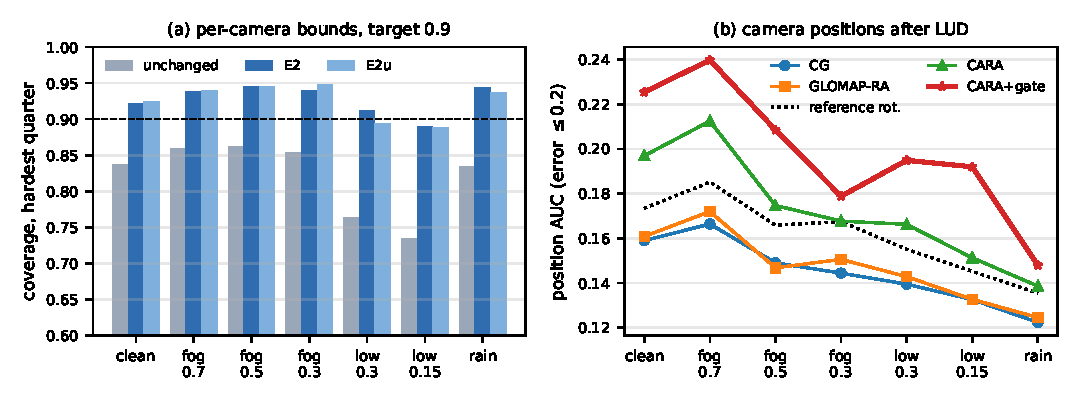
\includegraphics[width=\linewidth]{figs/v2.pdf}
\caption{Confirmatory ETH3D run (13 scenes). (a) Coverage of the per-camera bounds on the quarter of cameras with the largest $u_i$, for the unchanged bounds and the difficulty-conditional variants E2 and E2u; dashed line: target. (b) Position AUC after translation averaging by least unsquared deviations (LUD) with each method's rotations; CARA+gate uses only CARA's accepted edges, and the dotted line uses the reference rotations with all edges.}\label{fig:v2}
\end{figure}

\begin{table}[!htbp]\centering\footnotesize
\caption{Downstream camera positions (E5): LUD translation averaging of VGGT's relative translations, rotated by each method's global rotations. AUC of the scale-free position error up to $0.2$ (higher is better) and its median (lower is better); +gate uses only CARA's accepted edges. GT rot.\ uses the reference rotations and all edges.}\label{tab:v2trans}
\setlength{\tabcolsep}{2pt}\resizebox{\columnwidth}{!}{\begin{tabular}{lcccccc}\toprule
 & GT rot. & CG & GLOMAP-RA & CARA & CARA+gate & CARA-L+gate \\\midrule
clean & 0.173/0.32 & 0.159/0.37 & 0.161/0.38 & 0.197/0.33 & 0.225/0.33 & 0.233/0.32 \\
fog 0.7 & 0.185/0.34 & 0.166/0.39 & 0.172/0.39 & 0.212/0.36 & 0.240/0.34 & 0.227/0.35 \\
fog 0.5 & 0.166/0.35 & 0.149/0.41 & 0.147/0.42 & 0.175/0.39 & 0.208/0.36 & 0.202/0.37 \\
fog 0.3 & 0.167/0.35 & 0.144/0.42 & 0.151/0.41 & 0.168/0.40 & 0.179/0.40 & 0.173/0.41 \\
low 0.3 & 0.155/0.33 & 0.139/0.41 & 0.143/0.42 & 0.166/0.37 & 0.195/0.38 & 0.186/0.39 \\
low 0.15 & 0.145/0.35 & 0.133/0.44 & 0.133/0.44 & 0.151/0.40 & 0.192/0.39 & 0.178/0.41 \\
rain & 0.135/0.36 & 0.122/0.41 & 0.125/0.41 & 0.139/0.39 & 0.148/0.40 & 0.155/0.39 \\
\bottomrule\end{tabular}}\end{table}


\paragraph*{E5: effect on camera positions} We rotate VGGT's relative translations by each method's global rotations and solve translation averaging by least unsquared deviations (LUD)~\cite{ozyesil2015robust} on the same graph, then align to the reference centres by a similarity and divide the error by the median distance of the cameras to their centroid. \Cref{tab:v2trans} and \cref{fig:v2}(b) show that all methods give large position errors on these 12-camera graphs (median $0.32$ to $0.44$ of the scene radius), because many VGGT translation directions are wrong. CARA's rotations alone raise the position AUC over CG on all 13 scenes ($+0.028$, $p=0.0002$), partly because edges of unregistered cameras are dropped, and restricting LUD to CARA's accepted edges adds another $0.026$ (9 of 13 scenes, $p=0.073$). Together the gain over CG is $+0.053$ (12 of 13 scenes, $p=0.0005$), and the AUC exceeds that obtained with the reference rotations on all edges ($0.225$ against $0.173$ on clean scenes), so removing edges matters as much as correcting rotations. These AUC comparisons were not pre-registered. On the median position error, CARA with its gate is better than CG on 9 of 13 scenes ($p=0.030$), but not better than the reference rotations.

\begin{table}[!htbp]\centering\footnotesize
\caption{Pre-registered hypotheses for the confirmatory run. Difference averaged over the 13 test scenes, scenes in favour, exact sign-flip $p$ (one-sided for H1--H3 as pre-registered; two-sided for H4--H6, whose sidedness was not pre-registered) and Holm-adjusted $p$ over H1--H6.}\label{tab:v2hyp}
\setlength{\tabcolsep}{2.5pt}\resizebox{\columnwidth}{!}{\begin{tabular}{llcccc}\toprule
 & Hypothesis & diff. & scenes & $p$ & $p_{\mathrm{Holm}}$ \\\midrule
H1 & E2 raises hard-camera coverage (degraded) & +0.110 & 11/13 & 0.0005 & 0.0024 \\
H2 & E2 raises overall coverage (degraded) & +0.031 & 7/13 & 0.0447 & 0.0894 \\
H3 & E2 normalizer ranks catastrophic cameras better than $u$ & +0.002 & 5/12 & 0.4160 & 0.4160 \\
H4 & learned $\hat\sigma$ raises CARA's AUC@5 & +0.020 & 11/13 & 0.0181 & 0.0723 \\
H5 & learned $\hat\sigma$ raises outlier AUROC & +0.172 & 13/13 & 0.0002 & 0.0015 \\
H6 & CARA+gate lowers median position error vs CG & +0.037 & 9/13 & 0.0298 & 0.0894 \\
\bottomrule\end{tabular}}\end{table}


\paragraph*{Pre-registered hypotheses} \Cref{tab:v2hyp} lists the six hypotheses. The pre-registration fixed one-sided tests for H1--H3 but did not state the sidedness for H4--H6, which are directional; we report the conservative two-sided values. With one-sided values, H4 and H6 would also survive Holm correction ($0.036$ and $0.045$). The guarantee of \cref{cor:group} concerns the three groups by $v_i$; H1 measures the top quarter by $u_i$, a related but different set. After Holm correction two hypotheses hold: E2 raises coverage of the hardest cameras (H1) and the learned uncertainty separates outlier edges better (H5). Three are supported at the unadjusted level but not after correction: overall coverage under E2 (H2), accuracy with the learned uncertainty (H4) and the position error with CARA's edge set (H6). H3, a better ranking of catastrophic cameras by the learned normalizer, fails.


\subsection{Label-free audit of uncertainty}\label{sec:audit}
The drift statistic can also audit uncertainties that come with a dataset. If per-axis standard deviations were correct, the normalized cycle angle of a clean triangle would follow a Maxwell ($\chi_3$) law to first order, so $\hat\kappa(p)=\operatorname{Q}_p(t)/\operatorname{Q}_p(\chi_3)$ estimates their scale error without reference poses. On synthetic scenes with known factors $1, 2.4, 5, 10$ and no outliers, $\hat\kappa(0.05)$ returns $1.00, 2.43, 4.95, 9.97$. With 20\% outlier edges it overestimates by $28\%$, which is the value \cref{prop:bracket} predicts: 49\% of triangles are then contaminated and $\operatorname{Q}_{0.05/0.51}(\chi_3)/\operatorname{Q}_{0.05}(\chi_3)=1.28$. We attempted to apply the audit to the rotation covariances released with~\cite{zhang2023revisiting} for Madrid Metropolis, but the relative rotations stored in that file disagree with the 1DSfM relative rotations for the same pairs by a median of about $29^\circ$ and do not close around cycles under either orientation convention, so we could not establish the frame in which the covariances are expressed. We therefore report no result for real covariances.

\begin{figure}[!htbp]
\centering
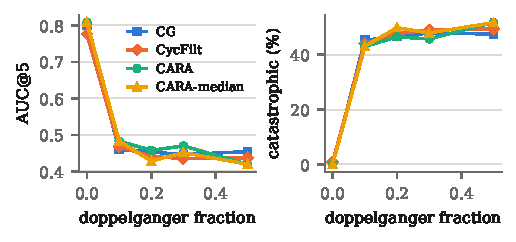
\includegraphics[width=\linewidth]{figs/dop.pdf}
\caption{Structured doppelgangers on a ring of 100 cameras around a symmetric object (5 seeds $\times$ 10 scenes per point). Spurious look-alike edges map a camera to its mirror twin and are mutually cycle-consistent. All methods fail once they are present.}
\label{fig:dop}
\end{figure}

\subsection{Structured doppelgangers}\label{sec:dop}
We place 100 cameras on a circle around an object with a $180^\circ$ symmetry and add spurious edges between cameras in the front half and cameras in the back half whose mirror twin would overlap them, with the relative rotation of the twin. These edges agree with each other around every cycle they share, so no cycle test can reject them. Without them, CARA reaches AUC@5 $0.808$ against $0.799$ for CG. With 10\% of the candidate look-alike pairs added (65 of 781 edges), every method fails: 43--45\% of cameras become catastrophic, CARA rejects only 12\% of the spurious edges, and bound coverage falls to 56\%. The picture does not change at higher fractions (\cref{fig:dop}). Neither the median triangle score nor the drift factor helps. This is the limit stated in \cref{rem:guar}: calibrated cycle tests do not replace doppelganger classifiers~\cite{cai2023doppelgangers,xiangli2025doppelgangerspp}, and the bounds are not valid when the error mechanism produces consistent wrong evidence.


